\documentclass[a4paper,11pt]{report}

\newdimen\largeur_1
\newdimen\largeur_2
\largeur_1 = \textwidth
\largeur_2= \textwidth
\divide\largeur_1 by 4
\divide\largeur_2 by 0.75

\usepackage[utf8]{inputenc}
\usepackage[T1]{fontenc}
\usepackage[french]{babel} 
\usepackage{lmodern}
\usepackage{makeidx}

\usepackage{fancyhdr}
\pagestyle{fancy}
\renewcommand{\headrulewidth}{1pt}
\fancyhead[LE]{\leftmark}
\fancyhead[LO]{\title}

\title{Automatisation de l'analyse d'incidents par l'utilisation du Machine Learning}
\author{\textsc{Lepont} Florian}
\date{\today} 

\title{Automatisation de l'analyse d'incidents par l'utilisation du Machine Learning}
\date{\today}
\author{Florian Lepont}
\makeindex

\begin{document}
	
\maketitle
\chapter*{Remerciements}
\thispagestyle{fancy}

Je tiens tout d'abord à remercier l'entreprise \emph{Aldebaran} de m'avoir accueilli et offert l'opportunité de réaliser mon stage ingénieur au sein de l'équipe "Qualification Hardware Pepper".

Je remercie tout particulièrement M Emmanuel Nalepa de m'avoir permis de participer à ce projet captivant et formateur, m'ayant ainsi permis d'étoffer mes connaissances dans plusieurs disciplines.  Sa disponibilité et sa pédagogie ont été des atouts essentiels à mon enrichissement technique.

J’adresse également mes remerciements aà toutes les personnes qui m’ont proposé leur aide durant ces vingt semaines :
M. Angelica Lim qui m’a fournie de précieuses informations, notamment dans le domaine du Machine Learning.

Je tiens enfin à remercier l'équipe "Qualification Hardware Pepper" pour l'aide qu'elle m'a apporté et sa très bonne humeur.

\begin{abstract}
\label{abstract}
Mon stage ingénieur, réalisé dans le cadre de ma cinquième année de formation à l'École Nationale d'Ingénieurs de Brest (ENIB), s’est déroulé au sein du département "Qualification Hadware Pepper (QWP) de l'entreprise Aldebaran. La société Parisienne s'est fait connaitre dans le monde des nouvelles technologies et de la robotique humanoïde grâce au développement de son premier produit, "Nao". A l'origine, le robot se prédestine à l'univers de la recherche et aux universités. La société cherche aujourd'hui à conquérir de nouveaux marchés en offrant des produits et des services au monde de l'entreprise et aux particuliers. Cela se traduit notamment par le développement d'un tout nouveau produit: "Pepper". 

Cette extension du marché s'accompagne d'une montée en puissance de la production des robots "Pepper". Cela induit le développement d'une nouvelle génération d'outils de production et post-production. Un des dispositif mis en place est le "Filtering Test": à la fin de la chaine de production, les robots sont soumis à une série de tests qui visent à mettre à l'épreuve les différentes parties mécaniques et électroniques. Lorsqu'une erreur est détectée,  les différentes données du robot son enregistrées (e.g. température des fusibles, valeurs de l'accéléromètre, etc.). Afin de déterminer qu'elles sont les causes qui ont entrainé l'apparition de l'anomalie sur le robot, chaque donnée est étudiée minutieusement et des hypothèses sont émises. Cette tâche dite d'investigation peu s'avérer laborieuse, le souhait d'automatiser ce processus est donc important.

Le but de  ma présence au sein d'Aldebaran est donc de répondre à ce besoin. En s'appuyant sur l'utilisation de méthodes d'apprentissage automatiques (en anglais, on parle de Machine Learning), j'ai donc mis au point un algorithme capable de déterminer automatiquement (après une phase d'apprentissage) les causes ayant entrainées l'apparition d'anomalies sur Pepper.  La mise au point de cet outil a été réalisé en trois temps:
\begin{enumerate}
	\item auto-formation à l'apprentissage automatique et de maitrise des outils.
	\item conception et développement de l'algorithme
	\item industrialisation du produit, c'est à dire en simplifier l'utilisation et le robustifier.
\end{enumerate}
 

Le rapport de stage ci-joint présente les différentes recherches effectuées ainsi que les travaux réalisés pour répondre au mieux à la problématique initiale.\end{abstract}

\tableofcontents
\listoffigures
\listoftables
\printindex
\chapter{Entreprise}
\label{Entreprise}
\thispagestyle{fancy}

\section{Histoire}
\label{Entreprise: histoire}
Aldebaran (anciennement Aldebaran Robotics) est une société française de robotique humanoïde fondée en 2005 par Bruno MAISONNIER.

\subsection{Le premier robot, NAO}
\label{Entreprise:Histoire:Nao}
Constituée au départ d'une équipe de douze collaborateurs, la toute jeune entreprise se fixe comme objectif de développer des robots humanoïdes et de les commercialiser au grand public en tant que "nouvelle espèce bienveillante à l'égard des humains". Après trois années de recherche et développement, la société dévoile en 2008 son tout premier produit: NAO. La participation du robot humanoïde à divers évènements internationaux, comme par exemple la RoboCup ou encore l'Exposition Universelle de Shanghai en 2010 participe à sa popularisation auprès des laboratoires de recherche, des universités et des développeurs. Une seconde génération de robot NAO apparait en 2011. L'entreprise dévoile durant la même période le projet Romeo dont l'objectif est de créer un véritable robot d'assistance à la personne, en partenariat avec différents acteurs de la recherche.

\subsection{La famille s'agrandit}
\label{Entreprise: La famille Aldebaran}
Lors de l'année 2012, Aldebaran Robotics est rachetée par SoftBank, société spécialisée dans le commerce électronique au Japon et prend le nom d'Aldebaran (suppression du terme "Robotics"). Débute alors la conception d'un tout nouveau produit, le robot humanoïde Pepper. Dévoilé au grand public en 2014, il est dans un premier temps vendu au Japon auprès des entreprises. Les premiers clients à en bénéficier sont les magasins de téléphonie mobile du groupe SoftBank. Les ventes s'ouvrent par la suite aux particuliers Japonais. La société compte aujourd'hui plus de 300 collaborateurs et poursuit le développement de ses trois produits afin de les améliorer et de conquérir de nouveaux marchés (Europe, Chine et États-Unis).

\section{Les produits}
\label{Entreprise: Les produits}
Aldebaran commercialise à ce jour deux produits: NAO et Pepper. Le robot Romeo est une plateforme de recherche.

\subsection{NAO}
\label{Entreprise: Les produits: Nao}
NAO est un robot humanoïde de 58 cm de hauteur. Les publics ciblés sont essentiellement les laboratoires de recherche et le monde de l'éducation (des écoles primaires jusqu'aux universités).

\begin{figure}[H]
	\centering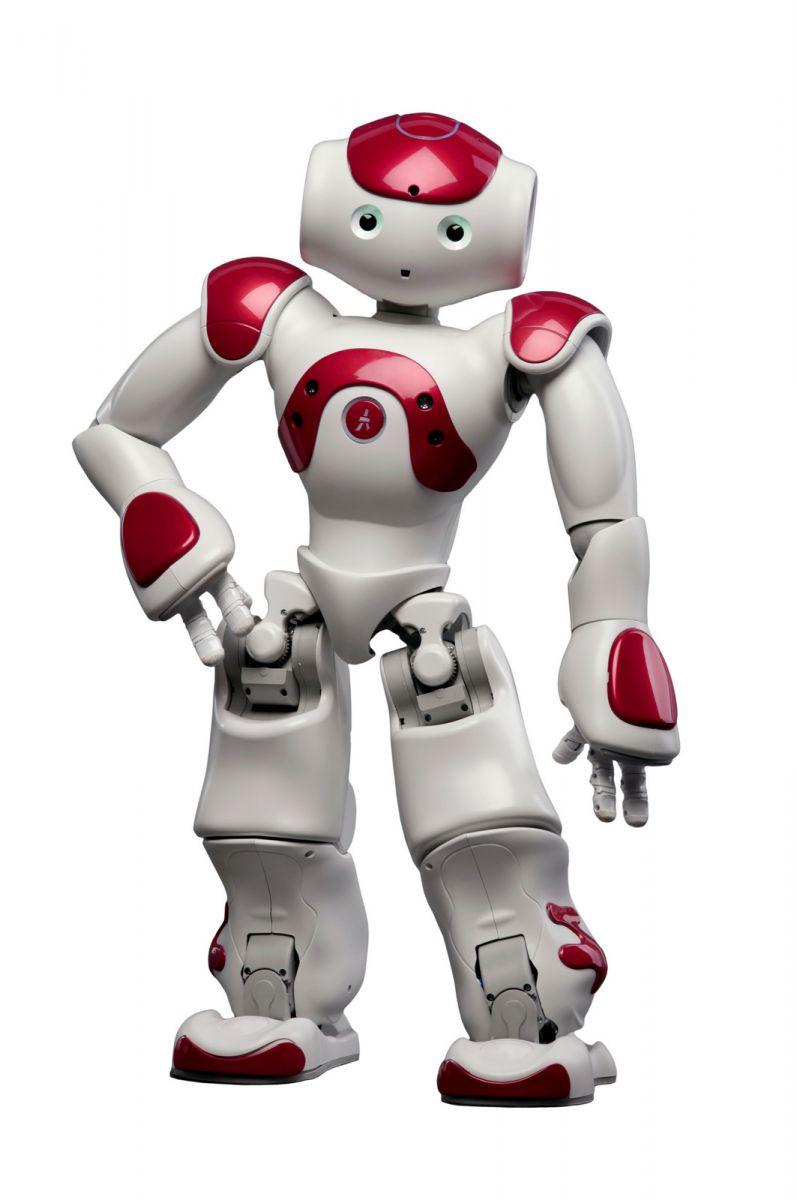
\includegraphics[height=7cm]{images/nao.jpg}
	\caption{Le robot humanoïde NAO}
	\label{fig:Robot humanoïde Nao}
\end{figure}

\paragraph{Caractéristiques techniques}
\label{Entreprise:Les produits: Nao: Caractéristiques techniques}
Caractéristiques techniques de la dernière version de Nao (V5, Évolution) tableau \ref{tab: Caractéristiques techniques de Nao}.

\begin{table}[H]
	\begin{tabular}{ | l | p{10cm} | }
	\hline
	\multicolumn{2}{|c|}{Caractéristiques générales} \\
	\hline
	Dimensions & 574 x 311 x 275 mm \\
	\hline 
	Masse & 5.4 kg \\
	\hline 
	Degrés de liberté  & 25 \\
	\hline
	Processeur & Intel Atom Z530 \newline 1.6 GHz \newline RAM: 1GB \newline Mémoire flash: 2GB  \newline Micro SDHC: 8 GB \\
	\hline
	Système d'exploitation & Middleware Aldebaran NAOqi basé sur un noyau Linux \\
	\hline
	Connectivité & Wi-Fi, Ethernet, USB \\
	\hline
	Batterie & Autonomie: 90 minutes en usage normal \newline Energie: 48.6 Wh \\
	\hline 
	Vision & Deux caméras frontales 2D, 1220p, 30ips \\
	\hline
	Audio & Sortie: 2 haut-parleurs stéréo \newline 4 microphones directionnels \newline moteur de reconnaissance vocale Nuance  \\
	\hline
	Capteurs & 2 capteurs infra-rouges, résistance sensible à la pression, centrale inertielle, 2 systèmes sonars, 3 surfaces tactiles \\
	\hline
	\end{tabular}
\caption[Caractéristiques techniques de NAO]{Caractéristiques techniques de la dernière version commerciale de NAO}
\label {tab: Caractéristiques techniques de Nao}
\cite{NaoTech}
\end{table}

\subsection{Pepper}
\label{Entreprise: Les produits: Pepper}
Dernier né d'Aldebaran, le robot Pepper est conçu pour vivre au côté des humains. Imaginé au départ pour accompagner et informer les clients dans les magasins de téléphonie du groupe japonais SoftBank, l'entreprise cherche à présent à placer son produit chez les particuliers. Le robot reprend la structure software et hardware de NAO. Contrairement à ce dernier, Pepper se déplace non pas grâce à une paire de jambes, mais via trois roues omnidirectionnelles qui facilitent son déplacement. A noter également que celui-ci est équipé d'une tablette tactile sur son torse pour faciliter les interactions Homme-Machine.

\begin{figure}[H]
	\centering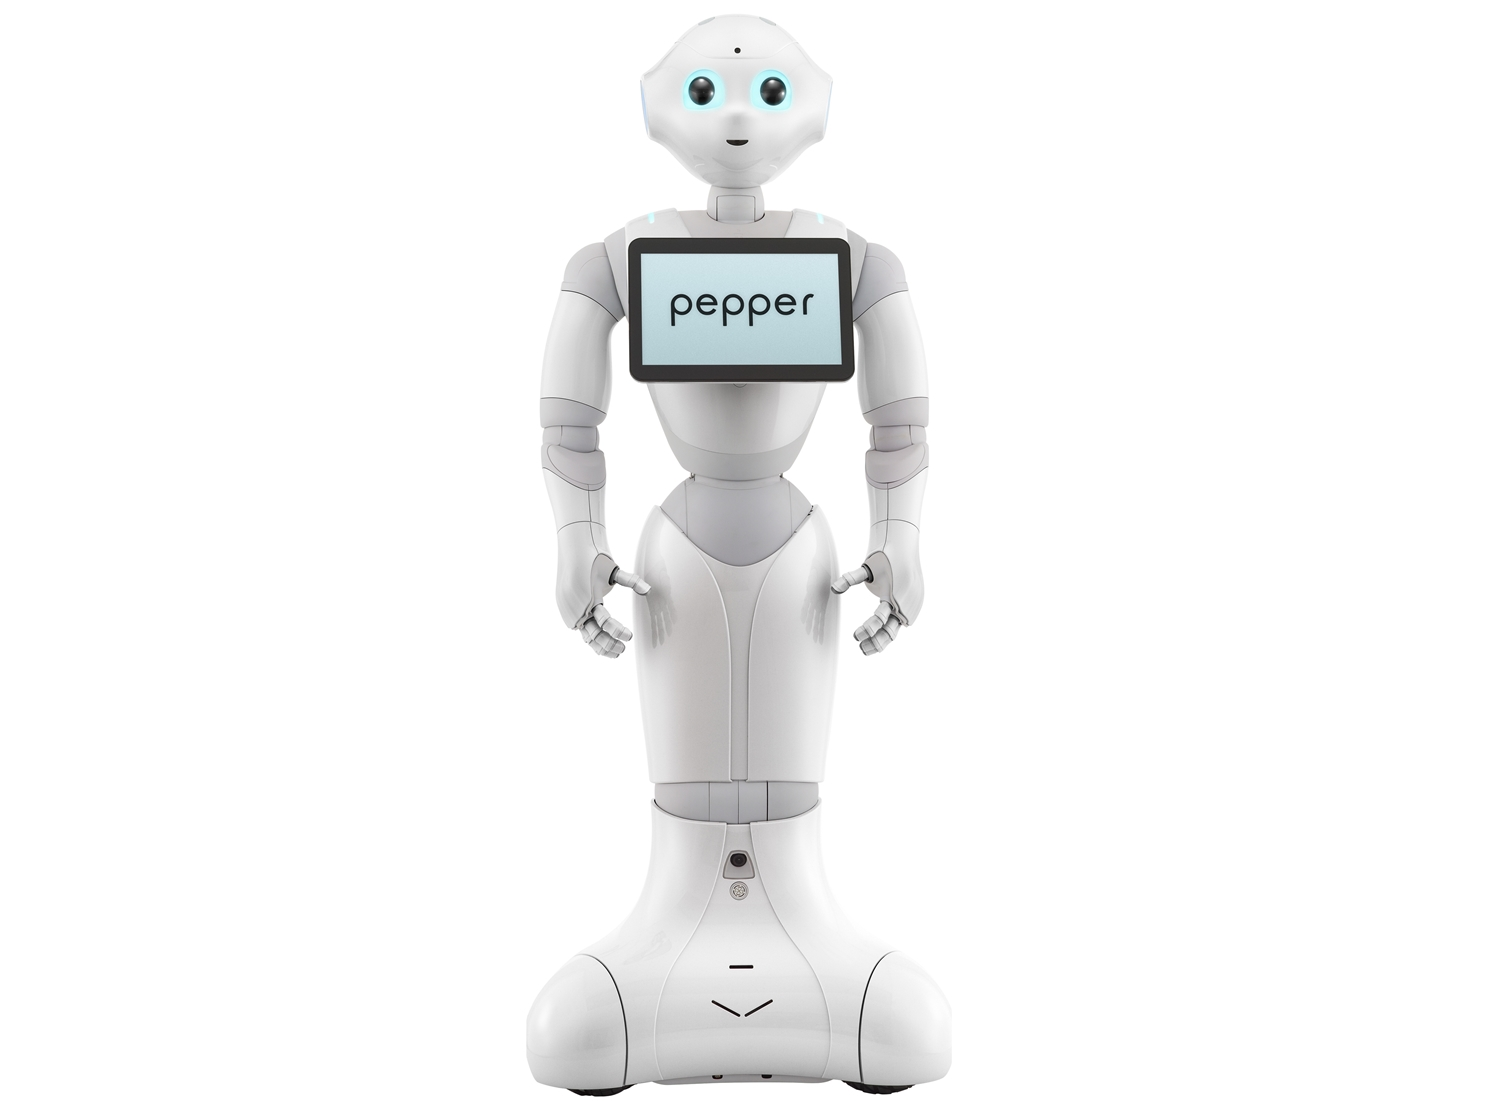
\includegraphics[height=6cm]{images/pepper.jpg}
	\caption{Le robot humanoïde Pepper}
	\label{fig:Robot humanoïde Pepper}
\end{figure}

\paragraph{Caractéristiques techniques}
Caractéristiques techniques de la dernière version commerciale de Pepper (V1.7) tableau \ref{tab: Caractéristiques techniques de Pepper}.

\begin{table}[H]
\begin{tabular}{ | l | p{10cm} | }
	\hline
	\multicolumn{2}{|c|}{Caractéristiques générales} \\
	\hline
	Dimensions & 1210 x 480 x 425 mm \\
	\hline 
	Masse & 28 kg \\
	\hline 
	Degrés de liberté  & 20 \\
	\hline
	Processeur & Intel Atom E3845 \newline 1.91 GHz \newline RAM: 4 GB \newline Mémoire flash: 8 GB \newline MICRO SDHC: 16Go  \\
	\hline
	Système d'exploitation & Middleware Aldebaran NAOqi,\newline basé sur un noyau Linux \\
	\hline
	Connectivité & Wi-Fi, Ethernet, USB \\
	\hline
	Batterie & Énergie: 795 Wh \\
	\hline 
	Vision & 2 caméras 2D \newline 1 caméra 3D \\
	\hline
	Audio & 3 microphones directionnels \newline moteur de reconnaissance vocale Nuance  \\
	\hline
	Connectivité & Wi-Fi, Ethernet \\
	\hline
	Capteurs & 6 lasers, 2 capteurs infra-rouges, 1 système sonar, résistance sensible à la pression, 2 centrales inertielles, 3 surfaces tactiles \\
	\hline
\end{tabular}
\caption[Caractéristiques techniques de Pepper]{Caractéristiques techniques de la dernière version commerciale  de Pepper}
\label {tab: Caractéristiques techniques de Pepper}
\cite{PepperTech}
\end{table}

\subsection{Romeo}
\label{Entreprise: Les produits: Romeo}
Romeo est un nouveau type de robot d'accompagnement et d'assistance à la personne. Cette plateforme de recherche est soutenue par Aldebaran ainsi que d'autres partenaires universitaires et laboratoires de recherche (e.g. INRIA, LAAS-CNRS, ISIR, ENSTA, Telecom, etc.). Il s'agit pour l'instant d'un prototype et sert principalement de plateforme de tests pour les prochaines innovations majeures d'Aldebaran (e.g. yeux mobiles, système vestibulaire, etc.).

\begin{figure}[H]
	\centering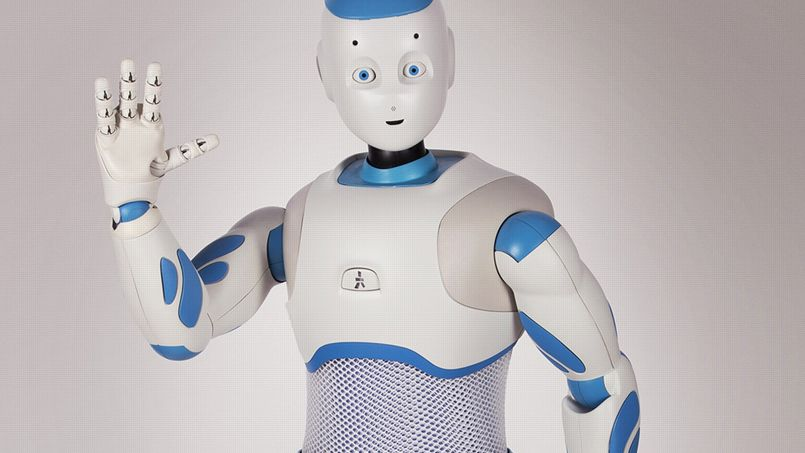
\includegraphics[height=6cm]{images/romeo.jpg}
	\caption{Le robot humanoïde Romeo}
	\label{fig:Robot humanoïde Romeo}
\end{figure}

\paragraph{Caractéristiques techniques}
Caractéristiques techniques de la dernière version commerciale de Romeo (V2) tableau \ref{tab: Caractéristiques techniques de Romeo}.

\begin{table}[H]
	\begin{tabular}{ | l | p{10cm} | }
		\hline
		\multicolumn{2}{|c|}{Caractéristiques générales} \\
		\hline
		Hauteur & 1467 mm \\
		\hline 
		Masse & 37 kg \\
		\hline
		Processeur & Intel ATOM Z530 \newline 1.6 GHz \newline RAM: 1 GB \newline Mémoire flash: 2 GB \newline MICRO SDHC: 8 Go  \\
		\hline
		Système d'exploitation & Middleware Aldebaran NAOqi,\newline basé sur un noyau Linux \\
		\hline
		Connectivité & Wi-Fi, Ethernet \\
		\hline
		Batterie & Énergie: 795 Wh \\
		\hline 
		Vision & 4 caméras 2D \newline 1 caméra 3D \\
		\hline
		Audio & 3 microphones directionnels \newline moteur de reconnaissance vocale Nuance  \\
		\hline
		Connectivité & Wi-Fi, Ethernet \\
		\hline
		Capteurs & 6 lasers, 2 capteurs infra-rouges, 1 système sonar, résistance sensible à la pression, 2 centrales inertielles, 3 surfaces tactiles \\
		\hline
	\end{tabular}
	\caption[Caractéristiques techniques de Romeo]{Caractéristiques techniques de la dernière version de Romeo}
	\label {tab: Caractéristiques techniques de Romeo}
	\cite{RomeoTech}
\end{table}

\subsection{Le système d'exploitation NAOqi}
\label{Entreprise: Les produits: NAOqi}
NAOqi est le système d'exploitation commun aux 3 robots d'Aldebaran. Il se base sur la distribution de Linux Gentoo et contient plusieurs APIs qui permettent de commander et contrôler les robots \cite{NAOqiTech}.
\begin{description}
	\item [NAOqi Core:] Gestion de l'ensemble des fonctions de base des robots (e.g. mémoire, "Autonomous Life", comportement du robot, etc.).
	\item [NAOqi Motion:] Gestion des mouvements du robot.
	\item [NAOqi Audio:]  Gestion de la partie audio du robot.
	\item [NAOqi Vision:] Gestion de la partie vidéo du robot.
	\item [NAOqi People Perception:] Ce module est utilisé pour détecter la présence de personnes autour du robot.
	\item [NAOqi Sensors:]  Gestion de l'ensemble des capteurs qui équipent le robot.
\end{description} 


\subsection{Plateforme de développement}
\label{Entreprise:Les produits: Nao: Plateforme de développement}
Les robots sont fournis avec une plateforme de développement.
\begin{description}
	\item[Choregraphe:] Il s'agit d'un outil de programmation graphique basé sur une interface qui prend la forme de schémas blocs \cite{ChoregrapheTech}. Il permet de façon simple d'interagir avec le robot et de concevoir des applications . Il peut s'utiliser avec un environnement de simulation 3D permettant aux développeurs de tester leurs applications sans même posséder un robot. Le logiciel permet également de disposer d'un retour visuel sur ce que le robot perçoit (e.g. vidéos issues des caméras, données des moteurs, etc.)
	
	\item[Kit de développement (SDK):] Il permet de développer des applications pour les robots via plusieurs langages de programmation:  C++, Python et Java \cite{SDKTech}.
\end{description}


\chapter{Introduction}
\label{Introduction}
\thispagestyle{fancy}

\section{Présentation du produit}
\label{Introduction:Présentation du produit}
On présente ici de manière succincte l'architecture Hardware du robot Pepper afin de se familiariser avec les différents éléments du système avec lesquels on sera susceptible de travailler durant la mise en œuvre de ce projet.  

\subsection{Les actionneurs}
\label{Introduction:Présentation du produit:Les actionneurs}
\subsubsection{Les moteurs}
\label{Introduction:Présentation du produit:Les actionneurs: Les moteurs}
Le robot Pepper est constitué de 20 moteurs dont il est possible de contrôler la position et la rigidité (figure \ref{fig:Répartition des actionneurs de Pepper})
\begin{description}
	\item [Tête:] 2 moteurs pour les mouvements de lacet (HeadYaw) et de tangage (HeadPitch)
	\item [Bras:] 4 moteurs par bras, répartis de la manière suivante: 
	\begin{description}
		\item [Épaule:] 2 moteurs pour les mouvements de tangage (ShoulderPitch) et de roulis du bras (ShoulderRoll).
		\item [Coude:] 2 moteurs pour les mouvements de roulis (ElbowRoll) et de lacet (ElbowYaw) de l'avant-bras.
	\end{description}
	\item [Main:] 1 moteur pour le mouvement de lacet du poignet (WristYaw) et 1 pour le mouvement d'ouverture et de fermeture de la main (Hand).
	\item [Hanche:] 2 moteurs pour le mouvement de roulis (HipRoll) et de tangage (HipPitch) du buste.
	\item [Genoux:] 1 moteur pour le mouvement de tangage (KneePitch) du haut du corps.
	\item [Roues:] 3 moteurs pour les mouvements de rotation de chacune des 3 roues omnidirectionnelles (WheelB, WheelFR et WheelFL).
\end{description}

\begin{figure}[h]
	\centering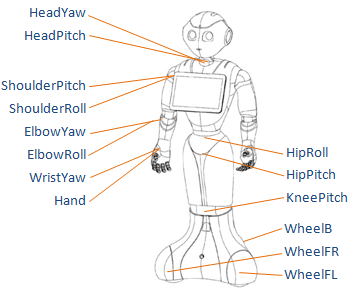
\includegraphics[height=7cm]{images/pepper_motors.png}
	\caption{Répartition des actionneurs de Pepper}
	\label{fig:Répartition des actionneurs de Pepper}
\end{figure}

\subsubsection{Les LEDs}
\label{Introduction:Présentation du produit:Les actionneurs: Les leds}
Les LEDs placées sur les épaules de Pepper, autour de ses yeux et de ses oreilles permettent d'obtenir un certain nombre d'informations sur son état. Par exemple, des LEDs bleues en rotations autour des yeux indiquent que le robot écoute.

\subsection{Les capteurs}
\label{Introduction:Présentation du produit:Les capteurs}
Pepper intègre également une multitude de capteurs. Certains d'entre eux sont utilisés pour s'assurer du bon comportement des parties mécaniques du robot, ou pour réaliser du contrôle-commande. D'autres capteurs sont en revanche intégrés sur le robot afin que l'utilisateur puisse interagir avec lui (tableau \ref{tab: Les différents capteurs de Pepper}).

\begin{table}[h]
	\begin{tabular}{ | p{3cm} | p{4cm} | p{7cm} | }
		\hline
		Capteur & Position & Description \\
		\hline
		Capteurs liés aux actionneurs & sur les moteurs & Chaque moteur du robot est lié à 3 capteurs, qui donnent des informations sur la valeur du courant délivré au moteur (A), la température du moteur (\degres C) et la position du moteur. \\
		\hline
		Capteurs tactiles & 1 sur chaque main, 3 sur la tête & Permet à l'utilisateur d'interagir avec le robot en le touchant.	\\	
		\hline 
		Les boutons & 1 bouton poussoir sur le buste, 3 bumpers sur la base & Les bumpers permettent au robot de détecter s'il rencontre un obstacle à proximité immédiate. Le bouton du buste permet quant à lui d'allumer le robot et de modifier le mode dans lequel il est (autonome, veille). \\
		\hline 
		Centrale inertielle & 1 dans le buste, 1 dans la base & Informe sur la position et l'orientation du robot, ainsi que la vitesse et l'accélération. \\
		\hline
		Sonars & 2 sonars à l'avant et l'arrière de la base & Permet de détecter la présence d'un objet situé au delà de 65 cm du robot. \\
		\hline 
		Capteurs batterie & batterie & Renseigne sur le courant et la tension délivrés, le pourcentage de charge et la température. \\
		\hline
		Capteurs infra-rouges & 2 sur la base &  Permet de détecter la présence d'un objet situé entre 0 et 50 cm du robot. \\
		\hline
		Lasers & 6 lasers sur la base du robot & Permet de détecter la présence d'un objet \\
		\hline 
	\end{tabular}
	\caption[Les différents capteurs de Pepper]{Les différents capteurs de l'architecture sensorielle de Pepper}
	\label {tab: Les différents capteurs de Pepper}
\end{table}


\section{Expression du besoin}
\label{Introduction:Expression du besoin}
L'extension du marché visée par Aldebaran pour Pepper s'accompagne d'une montée en puissance de la production. Afin de la guider, des outils de vérification des produits en fin de ligne de production sont mis en place. Parmi eux, on retrouve le "Filtering Test" qui consiste à réaliser une série de tests durant six heures. Il vise notamment à stresser l'ensemble des parties mécaniques du robot afin de faire ressortir d'éventuelles erreurs.

 \subsection{DExTER et MEIGUI}
 \label{Introduction:Expression du besoin:DExTER et MEIGUI}
 L'équipe de qualification hardware de Pepper a mis au point deux outils qui permettent de réaliser ces test et d'analyser les erreurs apparues.
 \begin{description}
 	\item[MEIGUI :] Le Filtering Test est réalisé grâce à MEIGUI. Celui-ci fait effectuer au robot un ensemble de mouvements qui permettent de stresser ses parties mécaniques. Si une anomalie survient lors du déroulement du test, les différentes données relatives à l'état des systèmes mécaniques et électroniques de Pepper sont enregistrées dans un fichier log, aussi appelé fichier journal en Français (e.g. température des fusibles, valeur des accéléromètres, etc.).
 	\item[DExTER :] Afin d'identifier les causes de l'apparition de problèmes sur le robot, un certain nombre d'hypothèses sont émises à partir de l'étude des données du fichier log. Pour cela, on s'appuie sur l'utilisation d'un autre outil, DExTER qui permet de visualiser les données du fichier log et d'obtenir des informations sur ces dernières (date d'apparition de l'erreur, nombre d'erreurs apparues, etc.).
 \end{description}
 
\subsection{Hiérarchisation des erreurs}
\label{Introduction:Expression du besoin:Hiérarchisation des erreurs}
Pour gérer au mieux les anomalies, celles-ci sont hiérarchisées en deux catégories: les \emph{errors name} et les \emph{root causes}.
\begin{description}
	\item [Error name] Cela correspond à l'erreur visible, i.e. la conséquence liée à une anomalie hardware ou software. Par exemple, il peut s'agir de la chute du robot. 
	\item [Root cause] Il s'agit de l'anomalie en elle même, i.e. la cause ayant entraînée l'apparition d'une \emph{error name}. Si l'\emph{error name} est la chute d'un robot, la \emph{root cause} peut par exemple être la détérioration d'un engrenage de la hanche.
\end{description} 

En suivant la logique exprimée par ces définitions, une \emph{error name} peut être constituée d'une ou plusieurs \emph{root cause}. 

\begin{table}
	\centering
	\begin{forest}
		for tree={
			draw,
			minimum height=2cm,
			anchor=north,
			align=center,
			child anchor=north
		},
		[{Chute du robot}, align=center, name=SS
			[{Engrenage cassé}, name=PDC]
			[{Courant des\\fusibles trop élevé}]
			[{Erreur sur la\\centrale inertielle}]
		]
		\node[anchor=west,align=left] 
		at ([xshift=-2cm]PDC.west|-PDC) {Level 2\\Root cause};
		\node[anchor=west,align=left] 
		at ([xshift=-2cm]PDC.west|-SS) {Level 1\\Error name};
	\end{forest}
	\caption[Exemple d'une error name et ses root causes]{Exemple d'un error name et ses root causes}
	\label {tab: Exemple d'un error name et ses root causes}
\end{table}

\subsection{Exemple d'analyse d'une anomalie}
\label{Introduction:Expression du besoin:Exemple d'analyse d'une anomalie}
On présente ici un exemple d'analyse d'un fichier log : 

\subsubsection{Observation}
\begin{itemize}
	\item Lors du déroulement du Filtering Test, le robot tombe à t = 16 972 secondes, soit lorsqu'il réalise une séquence de mouvements particulière appelée "Heat Behavior". Les valeurs retournées par l'accéléromètre selon l'axe $Z$ attestent de cette chute. (cf. figure \ref{fig:analyse d'une anomalie: accéléromètre})
	\item On analyse les données liées aux systèmes mécaniques et électroniques du robot qui peuvent avoir une relation directe ou indirecte avec sa chute.  Lorsque l'on étudie la vitesse de rotation du moteur de la hanche, on remarque qu'aux environs de  t = 16 970 secondes (c'est-à-dire 2 secondes avant la chute du robot), l'information fournie par le capteur ne suit plus la commande  envoyée au moteur (figure \ref{fig:analyse d'une anomalie: kneePitch}). On remarque également que le capteur du genou suit correctement la commande du moteur (cf. figure \ref{fig:analyse d'une anomalie: hipitch}).
	\item On observe aussi une augmentation anormale du courant dans le moteur de l'articulation de la hanche.
\end{itemize} 

\begin{figure}[h]
	\centering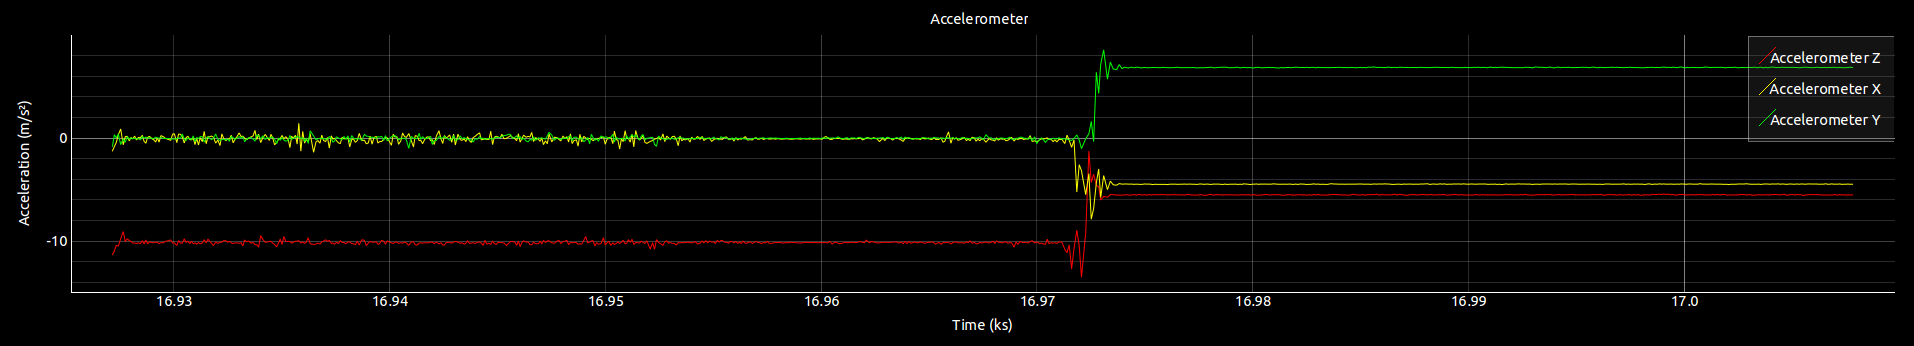
\includegraphics[width=15cm]{images/analyse_1.png}
	\caption{Analyse d'une anomalie: accéléromètre}
	\label{fig:analyse d'une anomalie: accéléromètre}
\end{figure}

\begin{figure}[h]
	\centering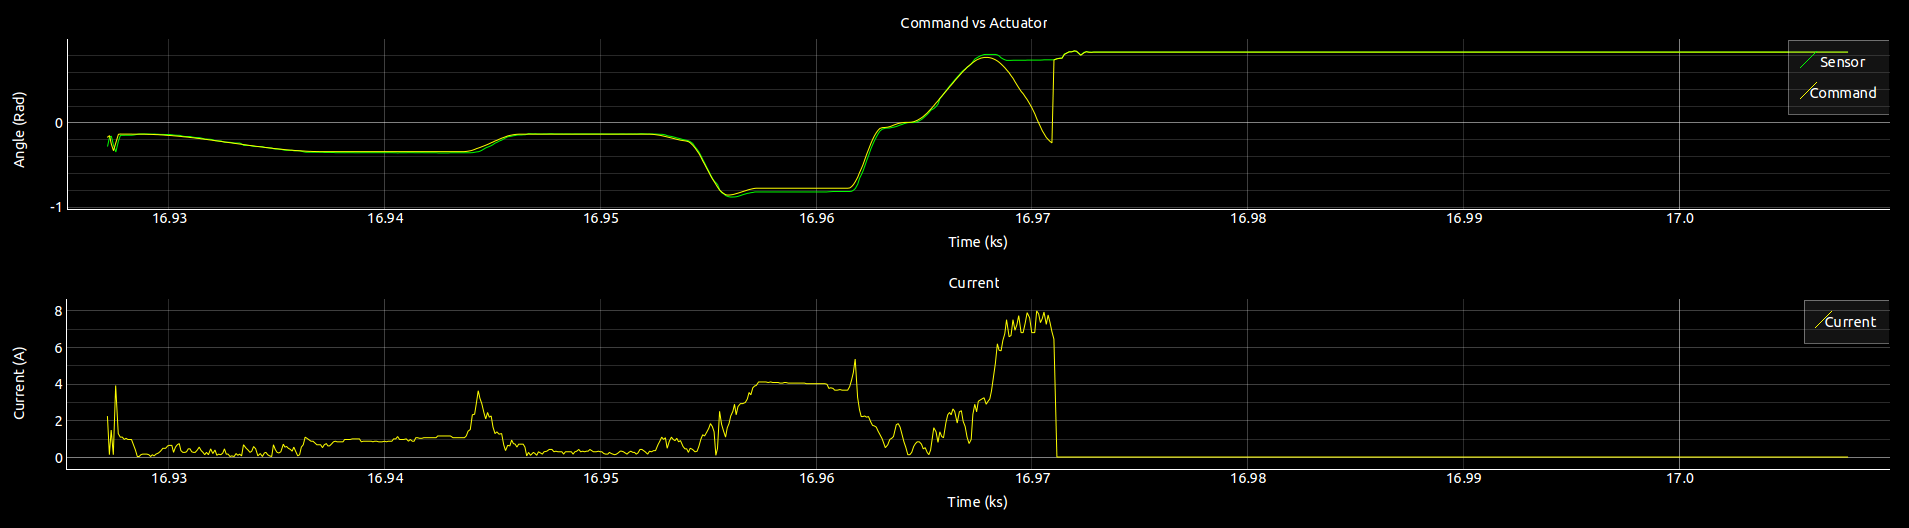
\includegraphics[width=15cm]{images/analyse_2.png}
	\caption{Analyse d'une anomalie: la hanche}
	\label{fig:analyse d'une anomalie: kneePitch}
\end{figure}

\begin{figure}[h]
	\centering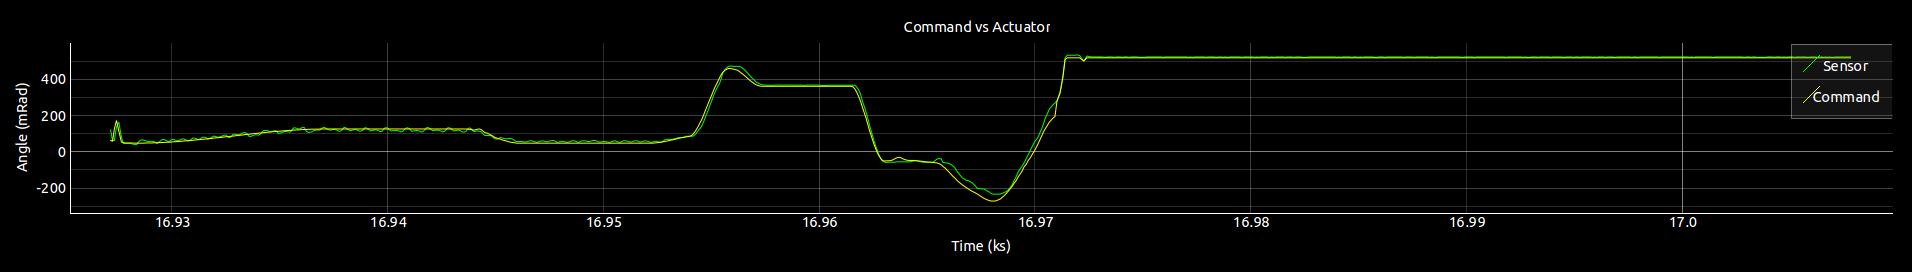
\includegraphics[width=15cm]{images/analyse_3.png}
	\caption{Analyse d'une anomalie: le genou}
	\label{fig:analyse d'une anomalie: hipitch}
\end{figure}

\subsubsection{Hypothèse émise}
 Lors de l'exécution de l'animation "Heat Behavior", le robot est amené à réaliser des mouvements amples au niveau de sa hanche qui causent un certain stress sur cette partie mécanique. Lorsque l'engrenage de la hanche arrive près de sa butée mécanique, un bloquage l'empêche d'atteindre sa position zéro. L'articulation de la hanche ne suit plus sa consigne, ce qui a pour effet de déséquilibrer le robot. Trop déséquilibré, Pepper tombe (\emph{error name}). Une étude plus poussée nous apprendra que la\emph{ root cause } du problème correspondait à un frottement du frein de la hanche. 


\section{Solution proposée}
De part la quantité d'informations à analyser, cette tâche d'analyse peut rapidement devenir rébarbative, d'où le souhait d'automatiser ce processus d'investigation. La variabilité des types de données nous empêche de réduire le nombre d'informations à analyser à de simples caractéristiques communes (e.g. moyenne, écart type, etc.). On s'appuiera donc sur des approches algorithmiques plus poussées, en utilisant notamment des méthodes d'apprentissages automatiques (plus connues sous le terme anglais de Machine Learning). La multiplicité des modèles englobés dans cette discipline nous permettra de répondre au mieux à la problématique.
chapter{Conclusion}
\label{Conclusion}
\thispagestyle{fancy}
\bibliographystyle{unsrt}
\bibliography{biblio}
\include {annexes}
\end{document}
